\chapter{Конструкторский раздел}

\section{Этапы решения поставленной задачи}

Исходными данными для задачи является описание диаграммы деятельности с помощью XMI. По этому описанию строится UML диаграмма и преобразуется в простую сеть Петри. Для построения раскрашенной сети из описания диаграммы выделяются используемые переменные, и строится предварительное описание типов. После задания пользователем начальной разметки на основе предварительных данных о типах переменных строится окончательное множество типов и раскрасок. И с учетом видимости переменных выстраивается раскраска сети. Общий процесс функционирования представлен на рис. \ref{fig:fig7}. 

\begin{figure}
	\begin{center}
		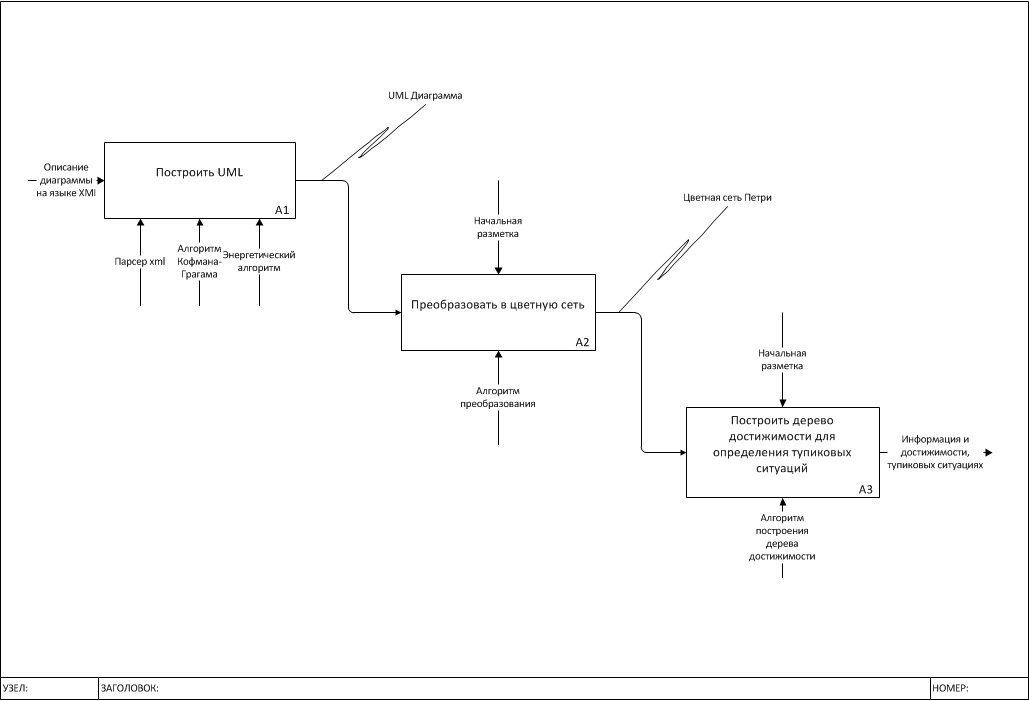
\includegraphics[width=\textwidth]{include/IDEF0.png}
	\end{center}
	\caption{Общий процесс функционирования.}
	\label{fig:fig7}
\end{figure}

Диаграмма деятельности представляет собой граф, вершины которого обозначают действия, а дуги ~--- переходы от одного действия к другому. Способы преобразования UML-диаграмм в простую сеть Петри широко известны, но для преобразования в раскрашенную сеть одних данных диаграммы не хватает: для раскрашенной сети необходимо сформировать множество типов и определить раскраски вершин (т.е. определить тип входных переменных). Процесс преобразования в раскрашенную сеть Петри представлен на рис. \ref{fig:fig8}.

\begin{figure}
	\begin{center}
		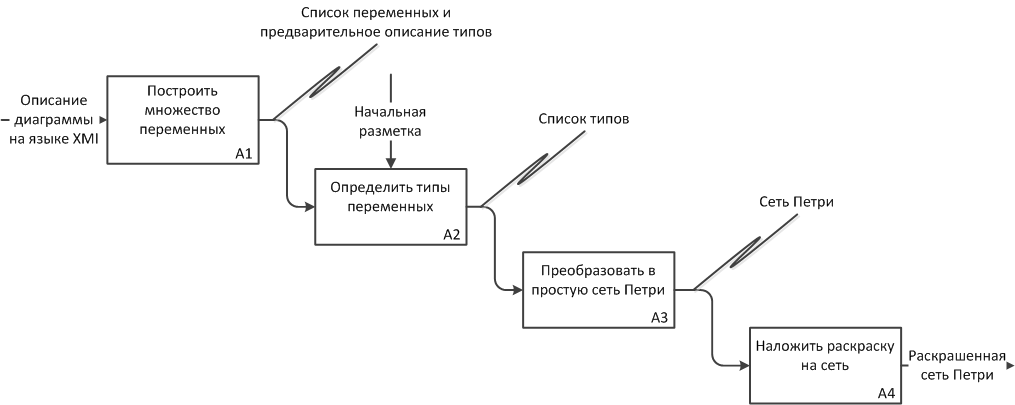
\includegraphics[width=\textwidth]{include/IDEF0ColoredPetri.png}
	\end{center}
	\caption{Процесс преобразования UML диаграммы деятельности в раскрашенную сеть Петри.}
	\label{fig:fig8}
\end{figure}

\section{Рисование бесконтурных графов}

Любую диаграмму деятельности можно свести к планарному графу, а значит и сеть Петри, построенную по этой диаграмме можно отобразить как планарный граф. Будем предполагать, что исходный бесконтурный граф является так называемым \textit{st-графом}, т.е. в нем имеется только одна начальная вершина, обозначаемая через \textit{s}, и одна конечная, обозначаемая через \textit{t}.

Аналитический алгоритм планарного представления графа описывает последовательность различных преобразований, приводящую к построению укладки. \cite{Battista} Краткий план работы алгоритма таков:
\begin{enumerate}
\item[1.] Построение ассоциированного орграфа G*.
\item[2.] Топологическая сортировка G и G*.
\item[3.] Мозаичное представление графа G.
\item[4.] Полилинейное изображение графа G, основанное на мозаичном представлении и информации о типах входных и выходных позиций.
\end{enumerate}

Рассмотрим каждый этап работы алгоритма подробнее.

\subsection{Построение ассоциированного орграфа G*}

Пусть G* ~--- планарный \textit{st-граф}, и пусть $ V, E и F $ - множества вершин, ребер и граней графа G, где внешние грани представлены в F двумя элементами $ s* $ и $ t* $, называемыми левой и правой внешней гранью G.
Определим орграф G*, ассоциированный с G, следующим образом:
\begin{itemize}
\item вершинами G* являются элементы из F;
\item для любой дуги $ e \neq (s, t) $ в G, граф G* имеет дугу $ e* = (f, g) $, где $ f $ ~--- левая по отношению к $ e $ грань, а $ g $ ~--- правая.
\end{itemize}

Для построения G* необходимо получить список всех граней графа G. Для данной задачи условимся понимать под гранью простой цикл графа, не содержащий в себе других циклов. Для поиска циклов используем модификацию алгоритма поиска в глубину:
\begin{verbatim}
function findBaseFaces(matrix, index, used[], track[]):
    used[index] = true;
    foreach outgoing vertex : v from vertex[index]:
        if not used[v]:
            track << v
            // Запуск поиска в глубину из текущей вершины.
            findBaseFaces(matrix, v, used, track)
            // Если вершина еще содержится в списке, то удаляем ее оттуда,
            // т.к. она не содержится в цикле.
            if (track.last = v)
                track remove last
        else if (track contains v) and (track.last <> v):
            // Берем вершины из списка пути следования
            // пока не встретится текущая вершина.
            previous = v;
            while v <> k:
                k << track
                faces << (previous, k)
                used[k] = not used[k]
                previous = k

            // Удаляем первую дугу цикла из графа, тем самым нарушая цикл,
            // и запускаем поиск из текущей вершины заново.
            (u, v) << faces.last
            matrix[u, v] = matrix[v, u] = 0
            continue cycle from begining
\end{verbatim}

Для поиска циклов необходимо преобразовать граф G в неориентированный граф простым симметричным отображением относительно главной диагонали. Алгоритм использует массив used для определения уже просмотренных вершин и список track, содержащий в себе вершины текущей итерации обхода. Если текущая вершина еще не была просмотрена, то запускаем поиск из нее, иначе, если эта вершина уже встречалась и это вершина не является предшественником текущей, мы нашли цикл.

Для нахождения всех вершин, содержащихся в цикле, мы забираем все вершины из списка track на пути до текущей, помечаем их как не пройденные, т.к. они могут содержаться в другом цикле, и добавляем дуги в список faces. После этого удаляем из графа первую дугу цикла. Так как поиск в глубину идет с лева на право, то если эта дуга содержится в другом цикле, то этот цикл уже был найден на предыдущих шагах. 

\begin{figure}
	\begin{minipage}[H]{0.49\linewidth}
		\center{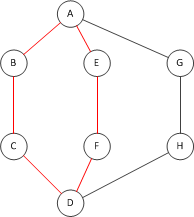
\includegraphics[scale=1]{include/RemoveCycles1.png} \\ Найден цикл (A,B) \rightarrow (B,C) \rightarrow (C,D) \rightarrow (D,F) \rightarrow (F,E) \rightarrow (E,A). \\ Удаляется первое ребро цикла (A,B).}
	\end{minipage}
	\hfill
	\begin{minipage}[H]{0.49\linewidth}
		\center{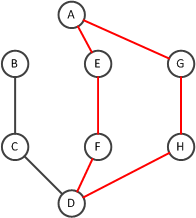
\includegraphics[scale=1]{include/RemoveCycles2.png} \\ Найден цикл (A,E) \rightarrow (E,F) \rightarrow (F,D) \rightarrow (D,H) \rightarrow (H,G) \rightarrow (G,A). \\ Удаляется первое ребро цикла (A,E).}
	\end{minipage}
	\hfill
	\begin{minipage}[H]{0.49\linewidth}
		\center{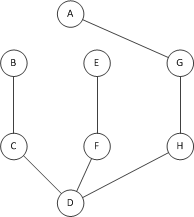
\includegraphics[scale=1]{include/RemoveCycles3.png} \\ Циклов больше нет.}
	\end{minipage}
	\caption{Демонстрация работы алгоритма поиска реберных граней.}
	\label{fig:fig11}
\end{figure}

На основе множества граней графа G необходимо для каждого ребра определить левую и правую грани (рис. \ref{fig:fig12}) и по ним построить граф G*. Для определения ориентации ребер воспользуемся тем, что номера вершин и переходов упорядочены, т.е. дуга $ 1 \rightarrow 2 $ будет раньше, чем дуга $ 1 \rightarrow 3 $. Отсюда следует, что для определения положения граней относительно ребра необходимо определить на правом или левом пути из истока лежит эта грань. Для определения истока необходимо найти на грани вершину, из которой есть только исходящие дуги, но воспользовавшись тем, что вершины упорядочены, можно утверждать, что истоком будет вершина с наименьшим номером. Получаем, что если ребро лежит на левом пути из истока в сток грани, то грань относительно этого ребра правая, иначе ~--- левая.

\begin{figure}
	\begin{minipage}[H]{0.49\linewidth}
		\center{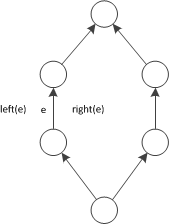
\includegraphics[scale=1]{include/EdgeOrientation.png}}
	\end{minipage}
	\hfill
	\begin{minipage}[H]{0.49\linewidth}
		\center{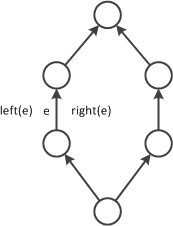
\includegraphics[scale=1]{include/VertexOrientation.png}}
	\end{minipage}
	\caption{Функции \textit{left} и \textit{right} для ориентированного графа.}
	\label{fig:fig12}
\end{figure}

Таким образом, получив для каждого ребра графа G левую и правую грань, выстраиваем матрицу смежности графа G* как переход из левой грани в правую. Матрица смежности G* понадобится в дальнейшем для топологической сортировки уровней G*, таким образом, нет нужды учитывать количество одинаковых дуг из одной грани в другую.

\subsection{Топологическая сортировка сетей}

Топологическая сортировка представляет собой алгоритм упорядочивания вершин бесконтурного ориентированного графа согласно частичному порядку, заданному ребрами орграфа на множестве его вершин. На первом шаге алгоритма мы выбираем все вершины с нулевой полустепенью захода, заносим их в нулевой уровень и исключаем их из графа. В результате, (больше не учитываются строки матрицы, соответствующие обработанным вершинам) полустепени захода остальных вершин уменьшатся. Шаги повторяются пока все вершины не будут просмотрены и распределены по уровням.

На рисунке \ref{fig:fig13} приведена итеративная работа алгоритма.

\begin{figure}
	\begin{minipage}[H]{0.99\linewidth}
		\center{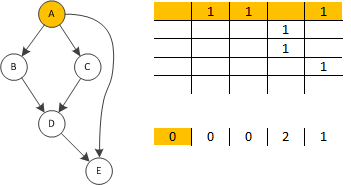
\includegraphics[scale=1]{include/TopologicalSort1.png} \\ Первая итерация. Вершина A не имеет входящих дуг.}
	\end{minipage}
	\vfill
	\begin{minipage}[H]{0.99\linewidth}
		\center{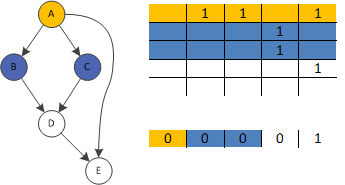
\includegraphics[scale=1]{include/TopologicalSort2.png} \\ Вторая итерация. Вершины B и С не имеют входящих дуг.}
	\end{minipage}
	\vfill
	\begin{minipage}[H]{0.99\linewidth}
		\center{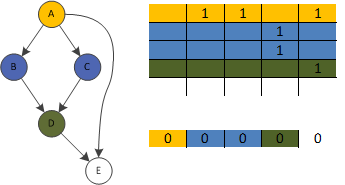
\includegraphics[scale=1]{include/TopologicalSort3.png} \\ Третья итерация. Вершина D не имеет входящих дуг. }
	\end{minipage}	
	\vfill
	\begin{minipage}[H]{0.99\linewidth}
		\center{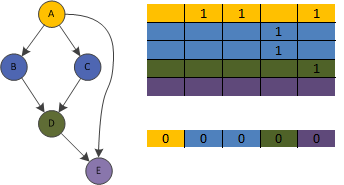
\includegraphics[scale=1]{include/TopologicalSort4.png} \\ Четвертая итерация. Вершина E не имеет входящих дуг. \\ Все вершины просмотрены, окончание работы алгоритма.}
	\end{minipage}
	\caption{Итеративная работа алгоритма топологической сортировки сети.}
	\label{fig:fig13}
\end{figure}

Если граф содержит цикл, то алгоритм на очередном шаге не сможет найти такую вершину, у которой полустепень захода равна нулю, другими словами, нельзя топологически представить цикл, т.к. для него нарушается правило $ X(p) > X(q) \Leftrightarrow (q, p) \epsilon E $.

\subsection{Мозаичное представление графа}

Мозаичное представление $ \Theta $ графа G ~--- это такое отображение каждого объекта $ O $ из $ V \bigcup E \bigcup F $ в плитку $ \Theta(O) $, что справедливы следующие свойства:
\begin{itemize}
\item если $ O_{1} \neq O_{2} $, то нет общих внутренних вершин у $ \Theta(O_{1}) $ и $ \Theta(O_{2}) $;
\item объединение всех плиток $ \Theta(O) $, $ O \epsilon V \bigcup E \bigcup F $ является прямоугольником;
\item $ \Theta(O_{1}) $ и $ \Theta(O_{2}) $ горизонтально инцидентны тогда и только тогда, когда $ O_{1} = left(O_{2}) , O_{1} = right(O_{2}) $ или $ O_{2} = left(O_{1}) , O_{2} = right(O_{1}) $;
\item $ \Theta(O_{1}) $ и $ \Theta(O_{2}) $ вертикально инцидентны тогда и только тогда, когда $ O_{1} = orig(O_{2}) , O_{1} = dest(O_{2}) $ или $ O_{2} = orig(O_{1}) , O_{2} = dest(O_{1}) $;
\end{itemize}

Вершины $ p \epsilon V $ графа G помечаются числами Y(p) таким образом, что Y(s) = 0 и $ Y(p) > Y(q) \leftrightarrow (q, p) \epsilon E $ ~--- дуга G.

Вершины $ p* \epsilon V* $ графа G* помечаются числами X(p*) таким образом, что X(s*) = 0 и $ X(p) > X(q) \leftrightarrow (q, p) \epsilon E* $ ~--- дуга G*.

Для каждой вершины вычисляются координаты горизонтального сегмента \ref{F:F1}:
\begin{equation}
	\begin{cases}
	y = Y(v) \\
	x_{1} = X(left(v)) \\
	x_{2} = X(right(v))
	\end{cases}
\label{F:F1}
\end{equation}

Для каждого ребра графа G вычисляются координаты вертикального сегмента \ref{F:F2}:
\begin{equation}
	\begin{cases}
	y = X(left(e)) \\
	x_{1} = Y(orig(e)) \\
	x_{2} = Y(dest(e))
	\end{cases}
\label{F:F2}
\end{equation}

\begin{figure}
	\begin{center}
		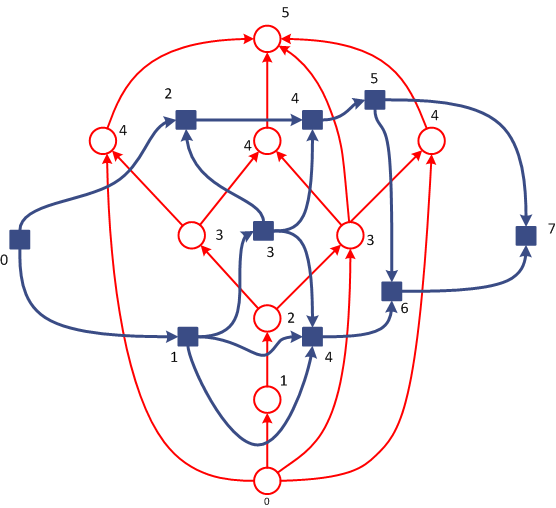
\includegraphics[scale=1]{include/Graph.png}
	\end{center}
	\caption{Планарный \textit{st}-граф G и ассоциированный граф G*.}
	\label{fig:fig14}
\end{figure}

\begin{figure}
	\begin{center}
		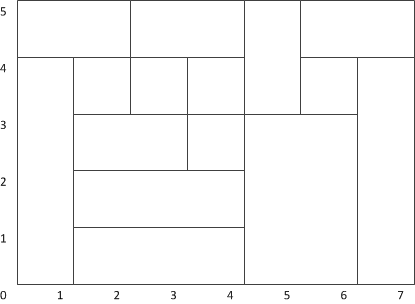
\includegraphics[scale=1]{include/MosaicView.png}
	\end{center}
	\caption{Мозаичное представление графа G.}
	\label{fig:fig15}
\end{figure}

Обзорным представлением Г заданного \textit{st-графа} G называется такое его изображение, в котором каждая его вершина p представлена горизонтальным отрезком Г(p), называемым вершинным отрезком, а каждая дуга (p, q) ~--- вертикальным отрезком Г(p, q), называемым реберным отрезком, таким образом, что справедливы следующие свойства:
\begin{itemize}
\item вершинные отрезки не накладываются друг на друга;
\item реберные отрезки не накладываются друг на друга;
\item реберный отрезок Г(p, q) имеет нижнюю границу, лежащую на Г(p), и верхнюю границу, лежащую на Г(q), и не пересекают ни один другой вершинный отрезок.
\end{itemize}

\subsection{Полилинейное изображение графа G}

Легко конструируется полилинейное изображение планарного \textit{st-графа} G на основе его обзорного представления. Для этого каждая вершина G может быть представлена некоторой точкой соответствующего вершинного отрезка, а каждая дуга (p, q) графа G ломанной, среднее звено которого образовано частью реберного отрезка, изображающего жту дугу (p, q).

Для каждой вершины заменить вершинный отрезок Г(v) на произвольную (среднюю) точку P(v) = (x(v), y(v)) отрезка Г(v).

Для каждого ребра (u, v), если это короткое ребро, т.е. расстояние y(v) - y(u) = 1, заменить реберный отрезок Г(u, v) на отрезок с конечными вершинами P(u), P(v). Иначе, если это ребро длинное, то заменить реберный отрезок Г(u, v) на ломаную линию, соединяющую точки P(u) и P(v) через точки $ (x(U(u, v)), y(u) + 1) $ и $ (x(Г(u, v)), y(u) - 1) $.

\begin{figure}
	\begin{center}
		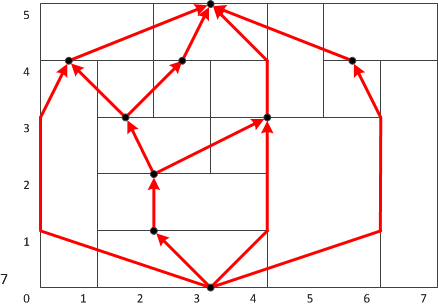
\includegraphics[scale=1]{include/PolylineView.png}
	\end{center}
	\caption{Полилинейное изображение графа G.}
	\label{fig:fig16}
\end{figure}

Наиболее оптимальное размещение точки P(v) ~--- это середина вершинного отрезка Г(v). При этом будет получаться плоское восходящее изображение, имеющее не более 6n - 12 сгибов, а каждое ребро имеет не более двух сгибов. При выборе позиции вершины P(v) в случае стратегии "выбора длинного ребра" можно размещать ее на внешней стороне вершинного отрезка и алгоритм будет строить полилинейное изображение графа в области размера $ O(n^{2}) $ с общим числом вершин $ (10 * n - 31) / 3 $ и не более, чем с двумя сгибами на одном ребре.

\section{Описание UML диаграмм с помощью XMI}

Для описания диаграммы деятельности используется стандарт XMI. Каждая вершина имеет имя, тип и уникальный идентификатор, описанные как атрибуты, и список входных и выходных вершин. Идентификатор используется для связи между вершинами и переходами. Если вершина имеет тип \textit{action}, то она может содержать описание действий, по которым в дальнейшем будет выстраиваться множество переменных.

Каждый переход имеет строго одну исходящую и входящую вершину и может содержать в себе правила защиты перехода (например, для условного перехода \textit{condition}).

Основываясь на описанных правилах, получим структуру описания диаграммы:

\begin{verbatim}
<activity_diagram>
    <states>
        <state id, name, type>
            <incoming transitions>
            <outgoing transition>
            <action>
        </state>
    </states>
    <transitions>
        <transition id>
            <source state>
            <target state>
            <guard>
        </transition>
    </transitions>
<activity_diagram>
\end{verbatim}

\section{Преобразование диаграммы деятельности в раскрашенную сеть Петри}

Наибольшей сложностью в процессе преобразования диаграммы в раскрашенную сеть Петри является формирование самой раскраски сети. Не существует четких правил, по которым можно определить достаточность раскраски, а так же возникает проблема избыточности, при которой сформированная сеть не будет точно моделировать работу диаграммы или не будет работать вовсе из-за невозможности совершения перехода.

Сам алгоритм построения раскрашенной сети Петри можно разделить на четыре этапа:
\begin{enumerate}
\item[1.] Выделение списка переменных для каждой вершины (рис. \ref{fig:fig17}).
\item[2.] Преобразование диаграммы деятельности в простую сеть Петри.
\item[3.] Введение начальной разметки и формирование типов для соответствующих переменных. Предварительное определение множества раскрасок (рис. \ref{fig:fig18}).
\item[4.] Определение максимальной области видимости переменных и формирование результирующей раскраски (рис. \ref{fig:fig19}).
\end{enumerate}

\begin{figure}
	\begin{minipage}[H]{0.49\linewidth}
		\center{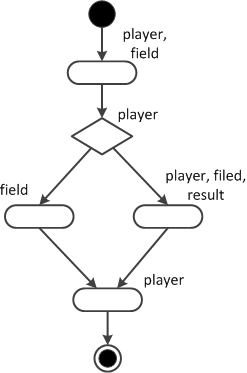
\includegraphics[scale=1]{include/ConvertVariables.png}}
		\caption{Выделение списка переменных.}
		\label{fig:fig17}
	\end{minipage}
	\hfill
	\begin{minipage}[H]{0.49\linewidth}
		\center{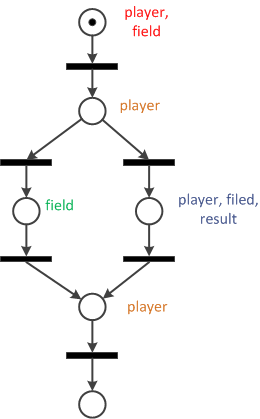
\includegraphics[scale=1]{include/ConvertDiagram.png}}
		\caption{Преобразование в простую сеть Петри и предварительное формирование множества раскрасок.}
		\label{fig:fig18}		
	\end{minipage}
\end{figure}

\begin{figure}
	\begin{minipage}[H]{0.8\linewidth}
		\center{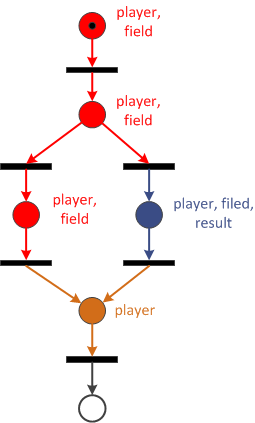
\includegraphics[scale=1]{include/ConvertColoring.png}}
		\caption{Формирование результирующей раскраски.}
		\label{fig:fig19}
	\end{minipage}	
\end{figure}

Исходя из общих правил формирования множества раскрасок, необходимо каждое составное действие разделить на объект, субъект и само действие (\ref{fig:fig9}).

\begin{figure}
	\begin{center}
		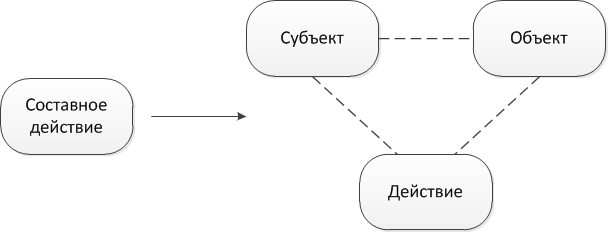
\includegraphics[width=0.6\textwidth]{include/CompositeActivity.png}
	\end{center}
	\caption{Треугольник сложного действия.}
	\label{fig:fig9}
\end{figure}

Сначала выделяются субъект и объект действия. Если на объект действия накладываются условные ограничения (не всегда может быть доступен, например, канал передачи данных, свободный блок оперативной памяти и т.п.), его необходимо отделить от субъекта действия, так как в сети Петри он будет обеспечивать второе условие для срабатывания перехода действия. Субъект и объект действия в общем случае связаны правилом, в соответствии с которым это действие происходит. \cite{Korotkov} 

\subsection{Получение списка переменных}

На первом этапе построение раскрашенной сети необходимо рассмотреть множество переменных, описывающих работу диаграммы. Условимся, что если переменные (в любой части описания переменной) имеют одинаковые имена, то они имеют и одинаковые типы.

На основе этого мы можем построить предварительное описание типов. Предположим, что на диаграмме имеются три блока действия:
\begin{verbatim}
player.cell = field.cell;
player.resource = player.resoure + field.resource;
player.resource = player.resoure - resource.
\end{verbatim}

По этому описанию можно заключить, что в системе фигурируют три переменные: player, field и resource, причем первые две имеют составной тип. Так же получаем то, что типы player и resource имет одинаковое описание типов: $ { cell, resource } $, причем тип всех переменных resource одинаковый. Таким образом, после первого этапа анализа получаем:

\begin{verbatim}
player : struct { cell, resource }
field : struct { cell, resource }
resource : simple type
\end{verbatim}

\subsection{Введение начальной разметки}

На втором этапе пользователю предлагается задать входные данные для диаграммы, основываясь переменных, выделенных на пером этапе. Основываясь на этих значениях, можно построить заключение о типах переменных. Остановим выбор на трех простейших типах: \textit{integer}, \textit{boolean}, \textit{string}, из которых можно образовывать кортежи и сложные структуры.

Для примера, приведенного на первом этапе, построим множество типов:

\begin{verbatim}
player : [ ((1, 1), 0) ]
field : [ ((1, 2), 2); ((1, 3), 1); ((2, 1), 1); ... ]
resource : 1
\end{verbatim}

Учитывая предварительное описание типов, получаем

\begin{verbatim}
player : struct { cell : (int * int), resource : int }
field : struct { cell : (int * int), resource : int }
resource : int
\end{verbatim}

Раскраска характеризуется кортежом типов. Так как каждая позиция содержит список переменных, на этом этапе можно сформировать предварительное множество раскрасок.

При введении начальной разметки значения переменных присваиваются первому вхождению этой переменной на пути из начальной вершины, а для остальных вершин, содержащих эту переменную, значения будут передаваться при функционировании системы с помощью фишек.

\subsection{Преобразование в простую сеть Петри}

Диаграмма деятельности во многом подобна сетям Петри. Но в сетях Петри действия моделируются переходами, а на диаграмме деятельности узлами. Кроме того, если в диаграмме деятельности движение фишки необходимо приостановить, то это делается между узлами на дугах, а не внутри блока. Таким образом, правильный перевод в сеть Петри заменяет узлы на переходы, а дуги на позиции. Узлы диаграммы представляются по-разному, в зависимости от типа (\ref{fig:fig10}):

\begin{figure}
	\begin{minipage}[h]{0.5\linewidth}
		\center{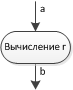
\includegraphics[scale=1]{include/Activity.png}}
	\end{minipage}
	\hfill
	\begin{minipage}[h]{0.4\linewidth}
		\center{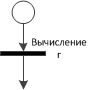
\includegraphics[scale=1]{include/ActivityPetri.png}}
	\end{minipage}
	\hfill
	\begin{minipage}[h]{1\linewidth}
		\begin{tabular}{ p{0.5\linewidth} p{0.5\linewidth} }
			\centering 1. & \centering 2. \\
		\end{tabular}
	\end{minipage}
	\hfill	
	
	\begin{minipage}[h]{0.5\linewidth}
		\center{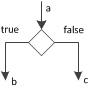
\includegraphics[scale=1]{include/Condition.png}}
	\end{minipage}
	\hfill	
	\begin{minipage}[h]{0.4\linewidth}
		\center{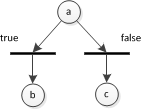
\includegraphics[scale=1]{include/ConditionPetri.png}}
	\end{minipage}
	\hfill
	\begin{minipage}[h]{1\linewidth}
		\begin{tabular}{ p{0.5\linewidth} p{0.5\linewidth} }
			\centering 3. & \centering 4. \\
		\end{tabular}
	\end{minipage}
	\hfill		
	
	\begin{minipage}[h]{0.5\linewidth}
		\center{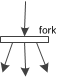
\includegraphics[scale=1]{include/Fork.png}}
	\end{minipage}
	\hfill	
	\begin{minipage}[h]{0.4\linewidth}
		\center{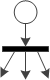
\includegraphics[scale=1]{include/ForkPetri.png}}
	\end{minipage}
	\hfill	
	\begin{minipage}[h]{1\linewidth}
		\begin{tabular}{ p{0.5\linewidth} p{0.5\linewidth} }
			\centering 5. & \centering 6. \\
		\end{tabular}
	\end{minipage}
	\hfill		
	
	\begin{minipage}[h]{0.5\linewidth}
		\center{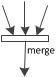
\includegraphics[scale=1]{include/Merge.png}}
	\end{minipage}
	\hfill
	\begin{minipage}[h]{0.4\linewidth}
		\center{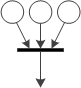
\includegraphics[scale=1]{include/MergePetri.png}}
	\end{minipage}
	\begin{minipage}[h]{1\linewidth}
		\begin{tabular}{ p{0.5\linewidth} p{0.5\linewidth} }
			\centering 7. & \centering 8. \\
		\end{tabular}
	\end{minipage}
	\hfill		
	
	\caption{Преобразование узлов диаграммы деятельности в сеть Петри.  деятельность; 3,4 условие; 5,6 ветвление; 7,8 синхронизация.}
	\label{fig:fig10}
\end{figure}

Условия для принятия решения в сетях Петри задаются как свойства соответствующих переходов. Позиция, предшествующая ветвлению, имеет два выхода, и маркер позиции перейдет через тот переход, условию которого удовлетворяет его значение. Стоит отметить потенциальную возможность ошибок, предупреждение которых целесообразно рассматривать как одно из формальных правил.
\begin{itemize}
\item Если для переходов ветвления не заданы условия их срабатывания, возникает неопределенность, в какую ветку перейдет маркер.
\item В случае если ни одно из условий не является истинным, переход становится недоступным ~--- маркер остается в своей позиции.
\end{itemize}

\subsection{Наложение раскраски}

На последнем этапе необходимо получить результирующую раскраску сети. На втором этапе была введена предварительная раскраска сети, основанная только на множестве переменных, принадлежащих вершине.

Для каждой переменной необходимо найти максимальную область ее видимости ~--- т.е. все возможные пути из вершины, где она встретилась в первый раз, до вершины, после которой она больше не содержится во множестве используемых переменных.

Основываясь на этом, мы расширяем список используемых переменных вершины и меняем ее раскраску.

\section{Обратная польская запись}

При переходе от диаграммы деятельности к раскрашенной сети Петри мы выделяем список переменных, на основе которых строится раскраска. При функционировании моделируемой системы переход сети может менять раскраску используемых фишек, а значит, и производить над ними вычисления. В связи с этим встает задача разбора и вычисления математических выражений. Как правило, арифметические выражения удобно преобразовывать в обратную польскую запись, чтобы избавиться от скобок, содержащихся в выражении. Выражения, преобразованные в польскую запись, можно вычислять последовательно, слева направо.

Отличительной особенностью обратной польской нотации является то, что все аргументы (или операнды) расположены перед знаком операции. В общем виде запись выглядит следующим образом:
\begin{itemize}
\item Запись набора операций состоит из последовательности операндов и знаков операций. Операнды в выражении при письменной записи разделяются пробелами.
\item Выражение читается слева направо. Когда в выражении встречается знак операции, выполняется соответствующая операция над двумя последними встретившимися перед ним операндами в порядке их записи. Результат операции заменяет в выражении последовательность её операндов и её знак, после чего выражение вычисляется дальше по тому же правилу.
\item Результатом вычисления выражения становится результат последней вычисленной операции.
\end{itemize}

Автоматизация вычисления выражений в обратной польской нотации основана на использовании стека. Алгоритм вычисления для стековой машины элементарен:
\begin{enumerate}
\item[1.] Обработка входного символа.
\begin{enumerate}
\item[1.1.] Если на вход подан операнд, он помещается на вершину стека.
\item[1.2.] Если на вход подан знак операции, то соответствующая операция выполняется над требуемым количеством значений, извлечённых из стека, взятых в порядке добавления. Результат выполненной операции кладётся на вершину стека.
\end{enumerate}
\item[2.] Если входной набор символов обработан не полностью, перейти к шагу 1.
\item[3.] После полной обработки входного набора символов результат вычисления выражения лежит на вершине стека.
\end{enumerate}

Реализация стековой машины, как программная, так и аппаратная, чрезвычайно проста и может быть очень эффективной. Обратная польская запись совершенно унифицирована ~--- она принципиально одинаково записывает унарные, бинарные, тернарные и любые другие операции, а также обращения к функциям, что позволяет не усложнять конструкцию вычислительных устройств при расширении набора поддерживаемых операций.

Существует несколько алгоритмов для превращения инфиксных формул в обратную польскую запись. Наиболее распространен переработанный алгоритм, идея которого предложена Э.В. Дейкстрой.

Для хранения переменных используется стек типа char.

Рассматриваем поочередно каждый символ:
\begin{enumerate}
\item[1.] Если этот символ - число (или переменная), то просто помещаем его в выходную строку.
\item[2.] Если символ ~--- знак бинарной операции (+, -, *, /), то проверяем приоритет данной операции. Получив один из этих символов, мы должны проверить стек:
\begin{enumerate}
\item[2.1.] Если стек все еще пуст, или находящиеся в нем символы имеют меньший приоритет, чем приоритет текущего символа, то помещаем текущий символ в стек.
\item[2.2.] Если символ, находящийся на вершине стека имеет приоритет, больший или равный приоритету текущего символа, то извлекаем символы из стека в выходную строку до тех пор, пока выполняется это условие; затем переходим к пункту 2.1.
\end{enumerate}
\item[3.] Если текущий символ - открывающая скобка, то помещаем ее в стек.
\item[4.] Если текущий символ - закрывающая скобка, то извлекаем символы из стека в выходную строку до тех пор, пока не встретим в стеке открывающую скобку, которую следует просто уничтожить. Закрывающая скобка также уничтожается.
\end{enumerate}

Если вся входная строка разобрана, а в стеке еще остаются знаки операций, извлекаем их из стека в выходную строку.

\section{Алгоритм построения дерева достижимости}

Алгоритм начинает свою работу с определения начальной разметки. До тех пор, пока имеются граничные вершины, они обрабатываются алгоритмом.

Пусть x – граничная вершина, которую необходимо обработать, и с которой связана разметка $ \mu(x) $.
\begin{enumerate}
\item Если в дереве имеется другая вершина y, не являющаяся граничной, и с ней связана разметка $ \mu(y) = \mu(x) $, то вершина x дублируется. 
\item Если для разметки $ \mu(x) $ ни один из переходов неразрешим, т.е. $ \mu(x) $ тупиковая разметка, то x терминальная вершина.
\item Для любого перехода $ t_{j} $, из множества T разрешенного в разметке $ \mu(x) $, создать новую вершину z дерева достижимости. Разметка $ \mu(z) $, связанная с этой вершиной, определяется для каждой позиции $ p_{i} $ следующим образом:
\begin{enumerate}
\item если $ \mu(x)_{i} = \omega, то \mu(z)_{i} = \omega $;
\item если на пути от корневой вершины к x существует вершина y такая, что $ \mu(y)\rightarrow^{t_{j}} \mu(x), \mu(y) < \mu(x) и \mu(y)_{i} < \mu(x)_{i} $, то $ \mu(z)_{i} = \omega $;
\item в противном случае $ \mu(z)_{i} = \mu(x)_{i} $.
\end{enumerate}

\end{enumerate}

Дуга, помеченная $ t_{j} $, направлена от вершины х к вершине z. Вершина x переопределяется как внутренняя, вершина z становится граничной. Когда все вершины дерева становятся терминальными, дублирующими или внутренними, алгоритм останавливается. Из алгоритма построения дерева достижимости следуют следующие выводы:
\begin{itemize}
\item сеть ограничена тогда и только тогда, когда символ $ \omega $ отсутствует в дереве;
\item сеть безопасна, если число фишек в каждой позиции не превышает 1;
\item сеть живая, если в дереве отсутствуют циклы и тупики.
\end{itemize}

\label{cha:design}
